\documentclass[a4paper,11pt,twoside]{article}

\usepackage{amsmath}
\usepackage{amssymb}
\usepackage[english]{babel}
\usepackage{cite}
\usepackage{color}
\usepackage{hyperref}
\usepackage{graphicx}
\usepackage{amsthm}
\usepackage{xspace}

\title{Assignment 3 -- literature overview}
\author{\href{mailto:pkok@science.uva.nl}{Patrick de Kok}}

% markup for geometric terminology
\newcommand{\textgt}[1]{\textsf{#1}\xspace} 
% geometric terminology
\newcommand{\pBrush}{\textgt{Brush}}
\newcommand{\pBrushes}{\textgt{Brushes}}
\newcommand{\ebrush}{\textgt{brush}}
\newcommand{\ebrushes}{\textgt{brushes}}
\newcommand{\pLine}{\textgt{Line}}
\newcommand{\pLines}{\textgt{Lines}}
\newcommand{\eline}{\textgt{line}}
\newcommand{\elines}{\textgt{lines}}
\newcommand{\pPencil}{\textgt{Pencil}}
\newcommand{\pPencils}{\textgt{Pencils}}
\newcommand{\epencil}{\textgt{pencil}}
\newcommand{\epencils}{\textgt{pencils}}

\newcommand{\pPlane}{\textgt{Plane}}
\newcommand{\pPlanes}{\textgt{Planes}}
\newcommand{\eplane}{\textgt{plane}}
\newcommand{\eplanes}{\textgt{planes}}
\newcommand{\pPoint}{\textgt{Point}}
\newcommand{\pPoints}{\textgt{Points}}
\newcommand{\epoint}{\textgt{point}}
\newcommand{\epoints}{\textgt{points}}
\newcommand{\pRegulus}{\textgt{Regulus}}
\newcommand{\pReguli}{\textgt{Reguli}}
\newcommand{\pRegPen}{\textgt{Regulus Pencil}}
\newcommand{\pRegPens}{\textgt{Regulus Pencils}}

% Math type specifying fonts
\newcommand{\V}[1]{\ensuremath{\mathbf{#1}}}

% Math-like symbols
\newcommand{\RL}{\ensuremath{\mathbb{R}^{3,3}}}
\newcommand{\en}{\ensuremath{\mathbin{\mbox{and}}}}
\newcommand{\of}{\ensuremath{\mathbin{\mbox{or}}}}
\newcommand{\eql}{\ensuremath{\Leftrightarrow}}

\newtheorem{theorem}{Theorem}
\newtheorem{question}{Question}
\newtheorem{lemma}{Lemma}

\definecolor{nicered}{rgb}{0.6, 0, 0.24}
\definecolor{nicegreen}{rgb}{0.0, 0.5, 0.24}
\definecolor{niceblue}{rgb}{0, 0.4, 1}

\hypersetup{
  colorlinks=true,
  urlcolor=nicegreen,
  linkcolor=niceblue,
  citecolor=nicered,
}

\begin{document}
\maketitle
\section{Research question and scientific significance}
With this bachelor thesis, I will try to give insight in the basis elements of the geometric algebra over $\RL$.  This will be accomplished by first investigating what the geometric interpretation of the basis elements in the space $\bigwedge \RL$.  After that, I will implement their visualisation in GAViewer.  

There are already several models of geometry in use in the geometric algebra community, of which the conformal model is the most popular and widely known~\cite{TheBook}.  Although usable in many cases, this model lacks the projective transformations.  The projective transformations are an important class of operations within computer vision and computer graphics.

Recently, researchers have found a way to express these transformations by using a 6 dimensional representation space with 3 basis vectors with squared norm $-1$~\cite{Hongbo}.  Using Pl\"ucker coordinates, lines are represented in the representational space by vectors with squared norm 0.  Different geometrical objects are generated by the outer product, which can be seen as linear algebra's $\operatorname{span}\{\}$ operator with linear properties.  For example, the outer product of two intersecting lines with a third line that intersects only one other line, represents a ruled surface.

GAViewer~\cite{GAViewer} is a visualisation and computing tool for the Euclidean and conformal models of geometric algebra, developed by Daniel Fontijne at the UvA.  These models contain other geometrical entities than the projective model.

In the original paper~\cite{Hongbo}, the authors haven't fully investigated what the geometrical meaning of the different elements of the algebra is.  I will show what geometrical entities are represented.  Afterwards, I will implement visualisations of these entities.

\section{Concept map}
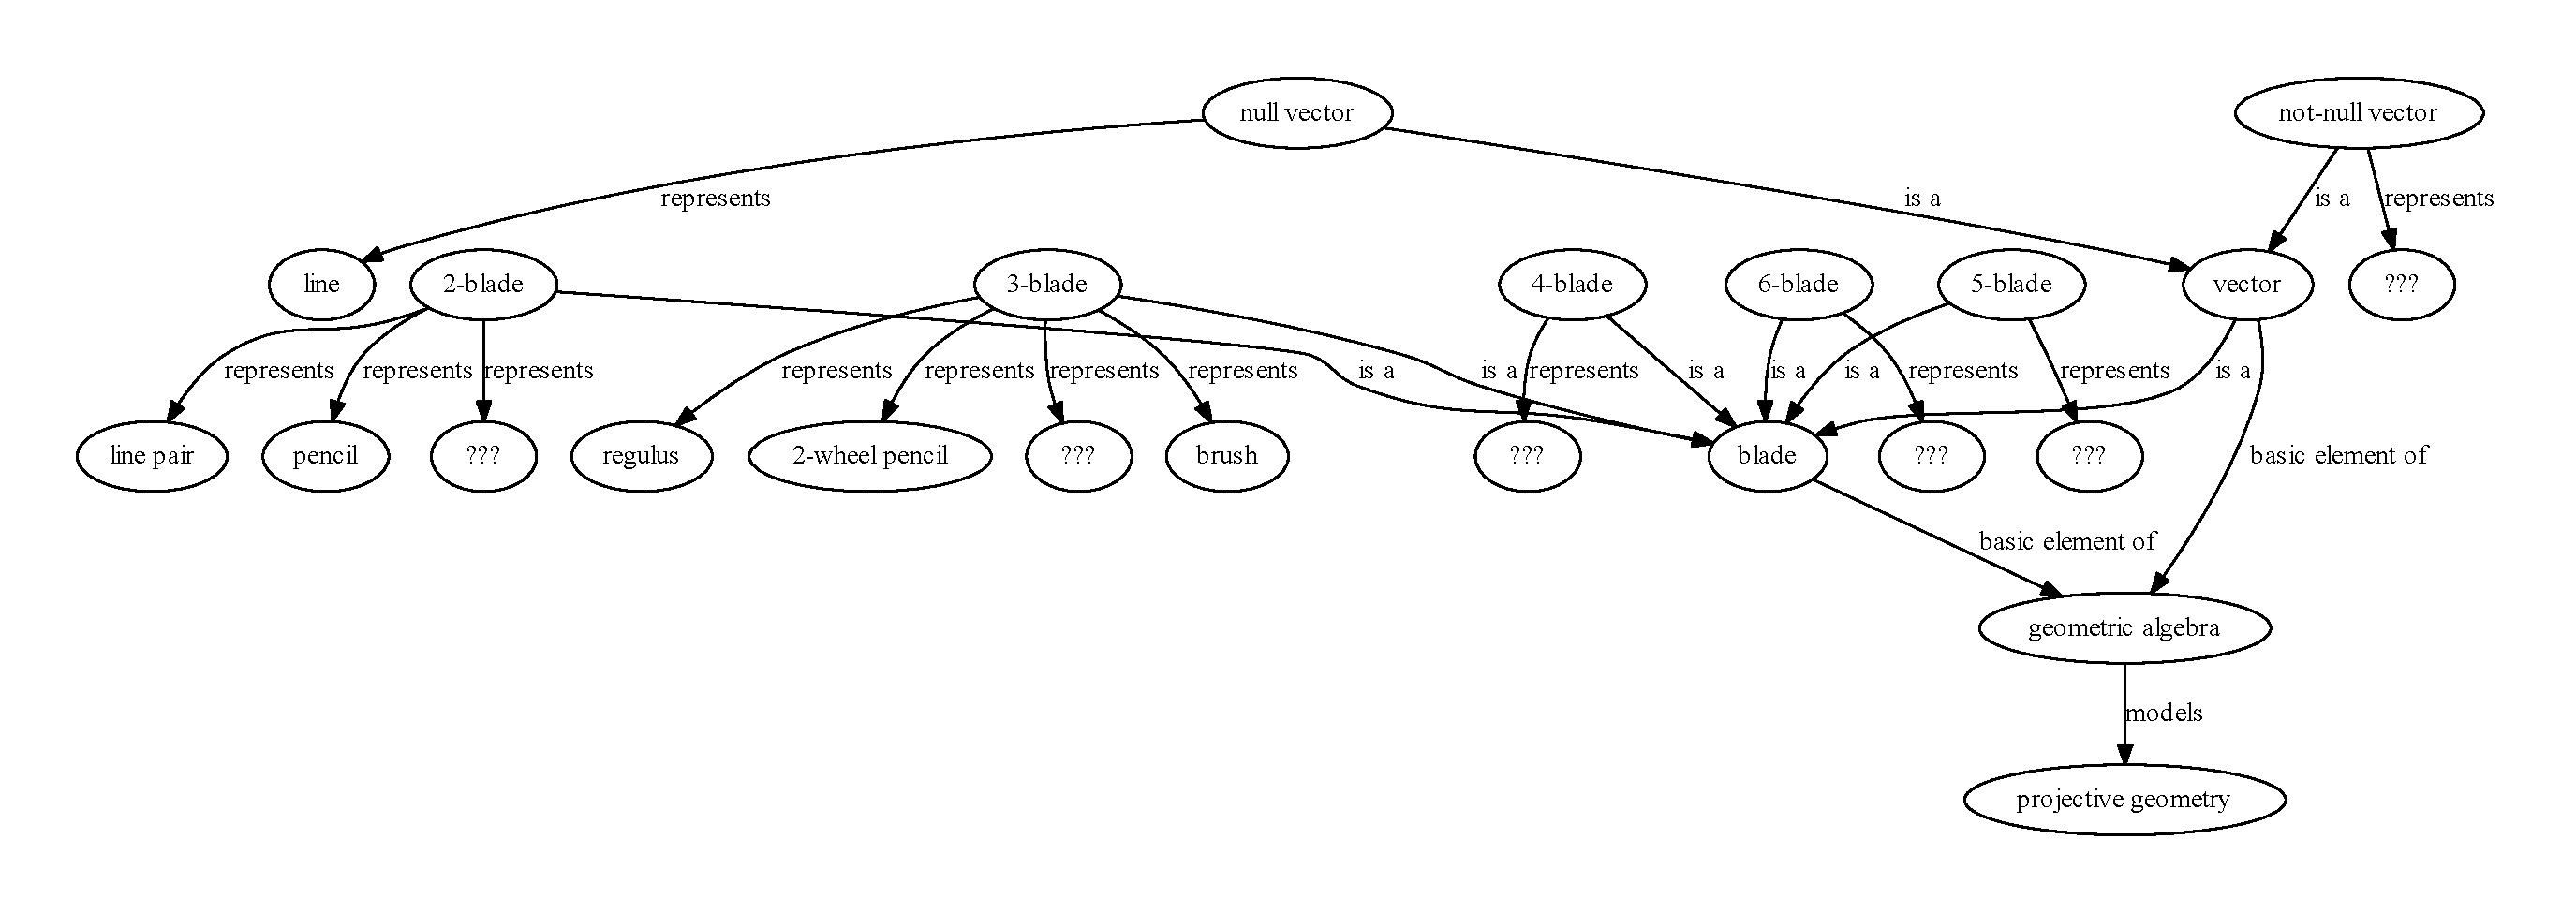
\includegraphics[width=1.0\textwidth]{conceptmap.pdf}

\section{Relevant articles}
For now, I only have found three relevant references.

\bibliography{citations}{}
\bibliographystyle{plain}
\end{document}
